\chapter{THỰC NGHIỆM KẾT QUẢ VÀ ĐÁNH GIÁ}
Qua các chương trước, luận văn đã trình bày thuật toán, lý thuyết cũng như cách thức hoạt động của chương trình nhận dạng ngôn ngữ ký hiệu. Ở chương này, luận văn sẽ trình bày kết quả thực nghiệm mà luận văn đã đạt được sau khi huấn luyện và các phương pháp đánh giá độ chính xác của mô hình.
\section{Thực hiện phần mềm nhận dạng ngôn ngữ ký hiệu}
Sau khi đã huấn luyện được mô hình nhận dạng ngôn ngữ ký hiệu, xây dựng thuật toán theo dõi đối tượng dựa trên Deep Sort. Tiếp theo, luận văn tiến hành xây dựng phần mềm nhận dạng thời gian thực để ứng dụng được mô hình đã huấn luyện trên ra thực tế.
\begin{itemize}
\item[$\square$] \textbf{Ngôn ngữ lập trình}
Python được sử dụng làm ngôn ngữ lập trình chính để xây dựng model cũng như viết ứng dụng nhận dạng.
\item[$\square$] \textbf{Thư viện Keras}
Thư viện Keras được sử dụng trong việc xây dựng model
\end{itemize}


\section{Kết quả}
Chương trình thực nghiệm đã nhận dạng được khá chính xác các hành động đã huấn luyện (16 ngôn ngữ ký hiệu). Chương trình chạy trên hệ điều hành ubuntu, sử dụng camera là webcam. Giao diện được viết trên thư viện PyQt5, là một thư viện hỗ trợ viết giao diện ứng dụng trên ngôn ngữ Python. Các nút điều khiển trên giao diện, giúp chọn các chế độ hoạt động của chương trình. Có tất cả 3 chế độ đều có thể hoạt động khi có nhiều người trong khung hình:
\begin{itemize}
\item Skeleton detection: Phát hiện và và trích đặc trưng khung xương từ camera.
\item Tracking: Theo dõi và đánh chỉ số của từng người trong khung hình dựa trên giải thuật Deep Sort.
\item Recognize: Theo dõi từng người và nhận dạng ngôn ngữ ký hiệu.
\end{itemize}
Giao diện và các mode hoạt động được trình bày như các hình \ref{fig:gui1}, \ref{fig:gui2}, \ref{fig:gui3}

\FloatBarrier
\begin{figure}[htp]
\begin{center}
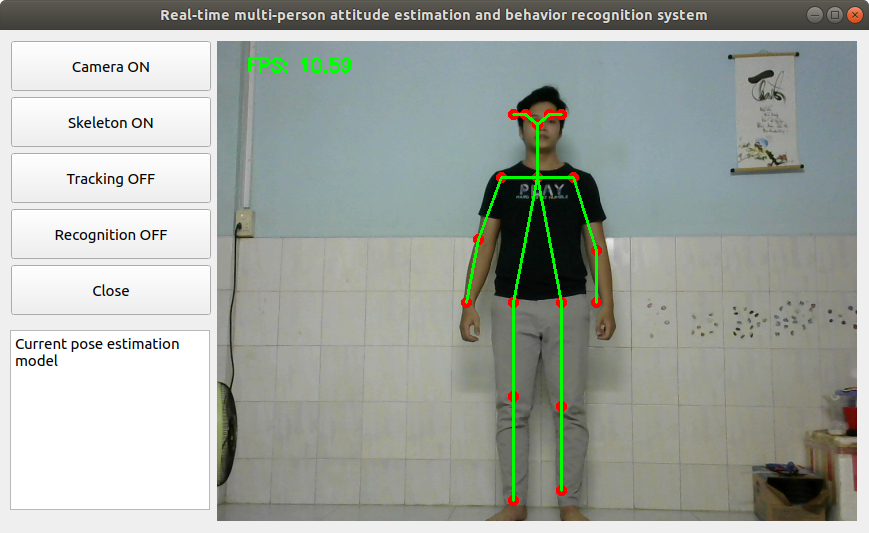
\includegraphics[scale=0.5]{chap6/c6_figs/mode_skeleton.png}
\end{center}
\caption{Giao diện phần mềm nhận dạng - Mode "Skeleton detection"}
\label{fig:gui1}
\end{figure}
\FloatBarrier

\FloatBarrier
\begin{figure}[htp]
\begin{center}
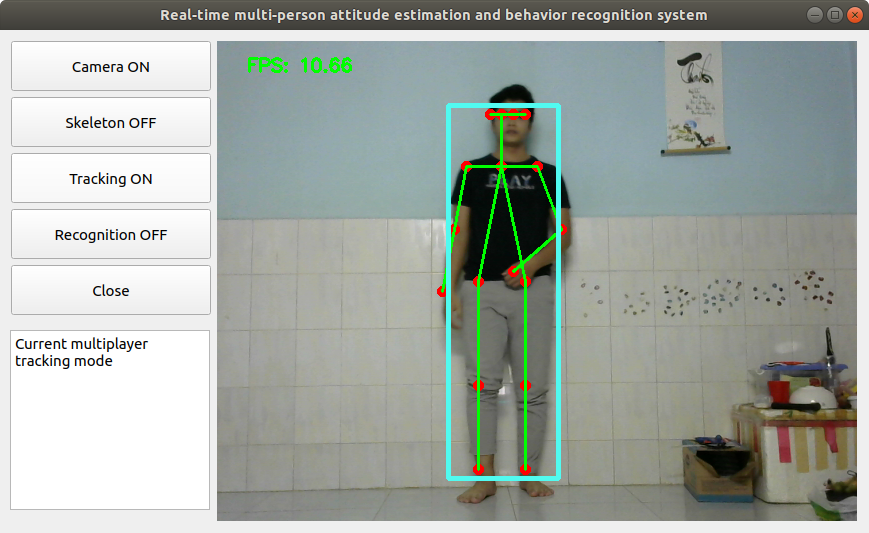
\includegraphics[scale=0.5]{chap6/c6_figs/mode_tracking.png}
\end{center}
\caption{Giao diện phần mềm nhận dạng - Mode "Tracking"}
\label{fig:gui2}
\end{figure}
\FloatBarrier

\FloatBarrier
\begin{figure}[htp]
\begin{center}
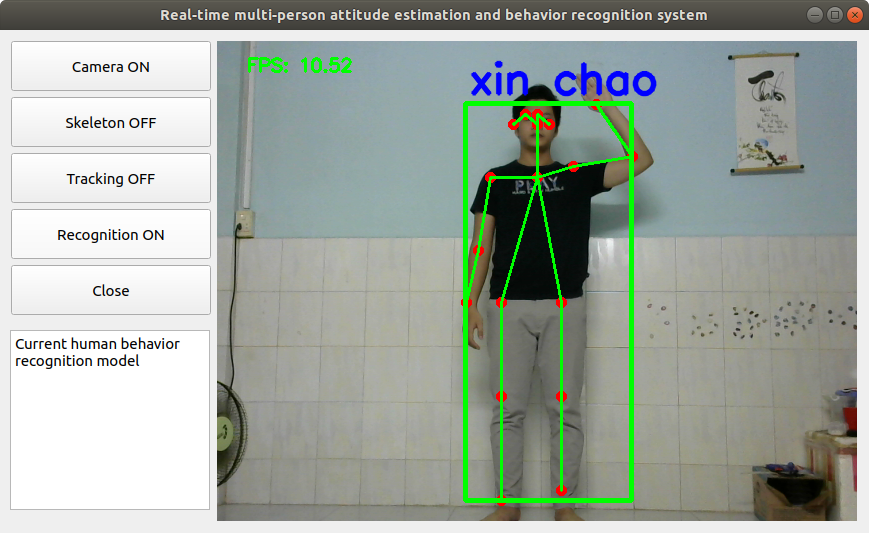
\includegraphics[scale=0.5]{chap6/c6_figs/mode_recognize.png}
\end{center}
\caption{Giao diện phần mềm nhận dạng - Mode "Recognize"}
\label{fig:gui3}
\end{figure}
\FloatBarrier

\section{Đánh giá}
Khi xây dựng một mô hình Machine Learning, chúng ta cần một phép đánh giá để xem mô hình sử dụng có hiệu quả không và để so sánh khả năng của các mô hình. Trong phần này, luận văn sẽ trình bày các mô hình classification.

Hiệu năng của một mô hình thường được đánh giá dựa trên tập dữ liệu kiểm thử (test data). Cụ thể, giả sử đầu ra của mô hình khi đầu vào là tập kiểm thử được mô tả bởi vector y-pred - là vector dự đoán đầu ra với mỗi phần tử là class được dự đoán của một điểm dữ liệu trong tập kiểm thử. Ta cần so sánh giữa vector dự đoán y-pred này với vector class thật của dữ liệu, được mô tả bởi vector y-true. Đối với bài toán phân loại của luận văn, có 16 lớp dữ liệu được gán nhãn là tên các từ được huấn luyện.


Có rất nhiều cách đánh giá một mô hình phân lớp. Tuỳ vào những bài toán khác nhau mà chúng ta sử dụng các phương pháp khác nhau. Các phương pháp thường được sử dụng là: accuracy score, confusion matrix, ROC curve, Area Under the Curve, Precision and Recall, F1 score, Top R error, etc.

Trong phần này, luận văn sẽ trình bày về accuracy score, confusion matrix, ROC curve, và Area Under the Curve. Và đánh giá mô hình của luận văn trên tập dữ liệu test gồm 400 SJM đối với mỗi từ.

\subsection{Accuracy}
Cách đơn giản và hay được sử dụng nhất là accuracy (độ chính xác). Cách đánh giá này đơn giản tính tỉ lệ giữa số điểm được dự đoán đúng và tổng số điểm trong tập dữ liệu kiểm thử.
\FloatBarrier
\begin{figure}[htp]
\begin{center}
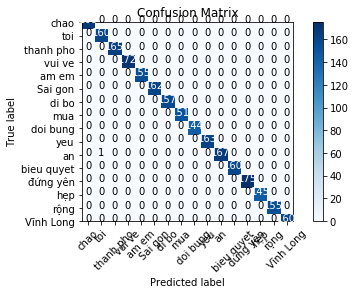
\includegraphics[scale=1]{chap6/c6_figs/confusion_matrix.png}
\end{center}
\caption{Confusion matrix của 16 lớp phân loại}
\label{fig:pipelineS}
\end{figure}
\FloatBarrier